\section{P1: Transformer depth}

\subsection{Learning rate sweeps}
Figure~\ref{fig:p1lr} and Table~\ref{tab:p1} summarise the 50 supplied transformer runs. The baseline d8 reaches 2.927 at $\lr=0.003$ and is flat within 0.02 over a factor of four in rate. Removing residual connections is fatal at every rate: all five runs sit at 6.875, the unigram level, so the model never learns to use its input. Removing pre-normalisation and post-norm both shift the usable rates down by a factor of three and lose 0.14 to 0.22 nats at their best rate; no-prenorm produces non-finite gradients at $\lr\geq 0.002$ and post-norm collapses at $0.004$. Removing QK normalisation costs little at the centre rate (2.951) but the loss explodes to 3.83 and 4.20 at $2\times$ and $4\times$ the centre: QK norm buys learning rate headroom rather than loss. Removing RoPE costs 0.14 nats at every rate, and removing the final norm costs 0.03 at the centre but degrades at high rates. The three gates all help a little: gated residuals 2.910, gated attention 2.917 and gated norm 2.939 (at its own centre of 0.00225, where the sweep is flat from 0.00225 to 0.009).

\begin{figure}[h]\centering
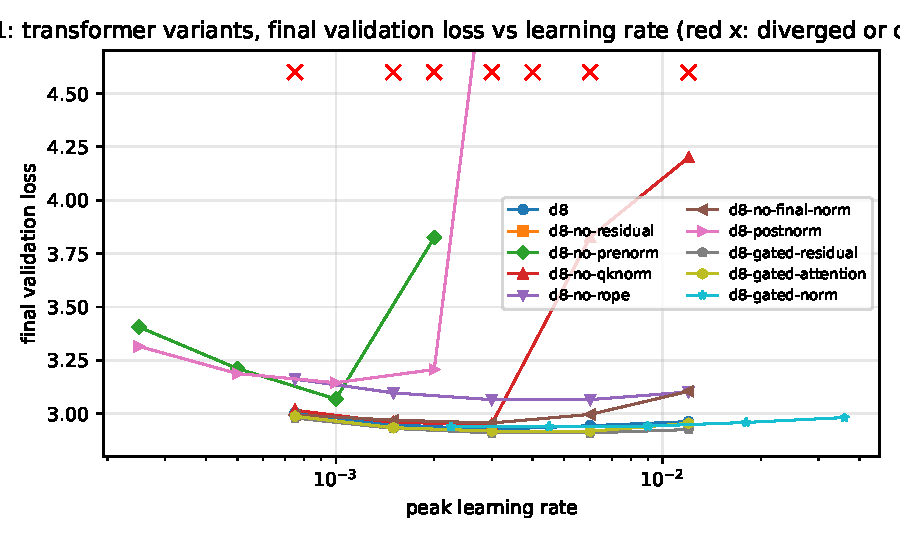
\includegraphics[width=.72\linewidth]{p1_lr_sweep.pdf}
\caption{P1 learning rate sweeps. Red crosses mark runs with non-finite gradients or final loss above 4.6 (no-residual at every rate sits at 6.875, off the axis).}
\label{fig:p1lr}
\end{figure}

\begin{table}[h]\centering\small
\caption{P1 final validation loss per rate (columns are $0.25\times$ to $4\times$ each variant's centre; best in bold; div. means non-finite). Params in millions.}
\label{tab:p1}
\begin{tabular}{lrrrrrrr}\toprule
variant & best $\lr$ & $0.25\times$ & $0.5\times$ & $1\times$ & $2\times$ & $4\times$ & params (M)\\\midrule
d8 & 0.003 & 3.004 & 2.948 & \textbf{2.927} & 2.943 & 2.963 & 34.6 \\
d8-no-residual & 0.00075 & \textbf{6.875} & 6.875 & 6.875 & 6.875 & 6.875 & 34.6 \\
d8-no-prenorm & 0.001 & 3.406 & 3.211 & \textbf{3.069} & 3.825 & div. & 34.6 \\
d8-no-qknorm & 0.003 & 3.016 & 2.959 & \textbf{2.951} & 3.827 & 4.200 & 34.6 \\
d8-no-rope & 0.003 & 3.162 & 3.097 & \textbf{3.065} & 3.066 & 3.101 & 34.6 \\
d8-no-final-norm & 0.003 & 2.994 & 2.969 & \textbf{2.956} & 2.996 & 3.104 & 34.6 \\
d8-postnorm & 0.001 & 3.315 & 3.188 & \textbf{3.145} & 3.207 & 6.875 & 34.6 \\
d8-gated-residual & 0.003 & 2.980 & 2.931 & \textbf{2.910} & 2.910 & 2.925 & 38.8 \\
d8-gated-attention & 0.006 & 2.987 & 2.934 & 2.918 & \textbf{2.917} & 2.955 & 34.6 \\
d8-gated-norm & 0.00225 & \textbf{2.939} & 2.940 & 2.941 & 2.959 & 2.982 & 38.8 \\
\bottomrule\end{tabular}

\end{table}

\subsection{Activation and gradient RMS across depth}
Figure~\ref{fig:p1depth} shows the FP32 probes of the final checkpoints at each variant's best rate, and Figure~\ref{fig:p1stages} tracks the baseline from initialisation to the end. In the baseline the residual stream RMS grows monotonically from 0.15 at the embedding to 24 before the final norm, with most of the growth in the first two blocks; the raw branch outputs are 6 to 20 times larger than their input at the first attention branch and then settle at 0.3 to 0.5 of the stream, so each later block is a small correction to a large stream. The gradient of the full loss with respect to the stream decays only from $1.4\times10^{-5}$ at the embedding to $3\times10^{-7}$ at the top and is nearly flat over the middle twelve branches, as the additive path guarantees; the last-token gradient is about 50 times larger (it is not averaged over 1023 targets) and has the same shape. The cosine between consecutive stream states is above 0.9 from block 2 onward: the stream changes direction mostly at the bottom. Training compresses the gradient range at the bottom (the embedding gradient falls by 1000 between init and step 100 while the top stays put), consistent with the first blocks growing the stream quickly.

The no-residual model is the opposite picture: at the final checkpoint the stream RMS grows from $2\times10^{-3}$ to 430 across 16 branches, the cosine between consecutive states is 0, and the gradient RMS spans $10^{-20}$ to $10^{-9}$ from bottom to top, so the lower half of the network is dead and the top learns a unigram predictor. The no-prenorm and post-norm models keep the stream between 0.05 and 1 but pay for it with gradients that are 10 to 100 times larger than the baseline's at every depth, which is why their rates had to be lowered. The no-final-norm model learns to keep its top stream at 1.4 instead of 24, because the head sees the raw stream. Gated residuals have the largest branch to input ratio (1.9 on average), meaning the gate lets the branches write more.

\begin{figure}[h]\centering
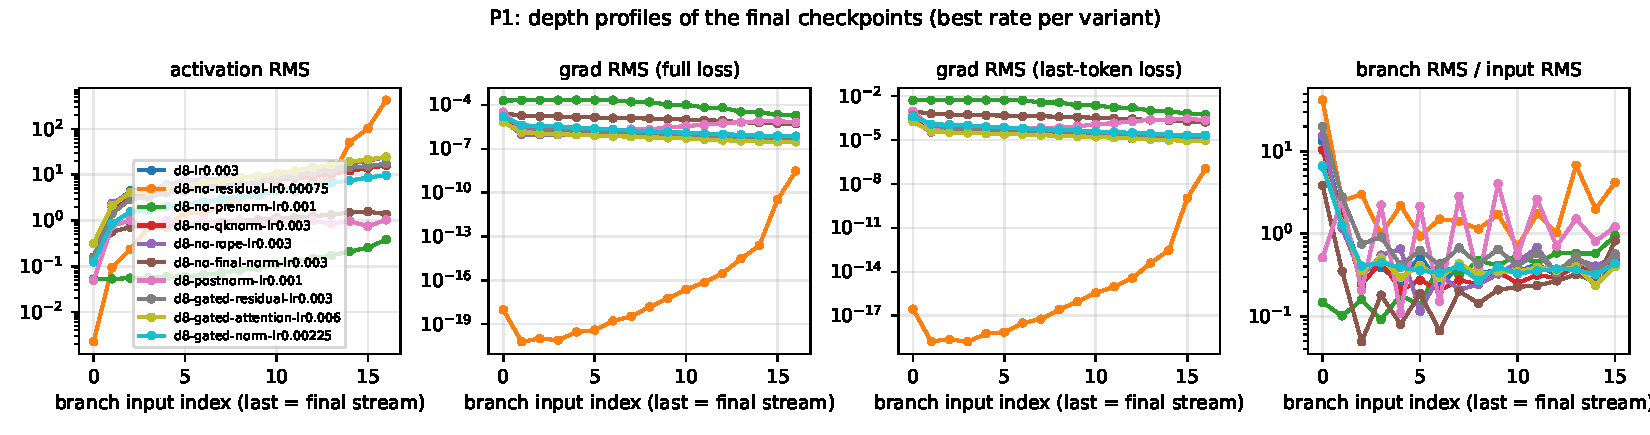
\includegraphics[width=\linewidth]{p1_depth_final.pdf}
\caption{P1 depth profiles of the final checkpoints. Index 0 is the embedding entering the first attention branch, odd indices are MLP branch inputs, index 16 is the final stream before the output norm.}
\label{fig:p1depth}
\end{figure}

\begin{figure}[h]\centering
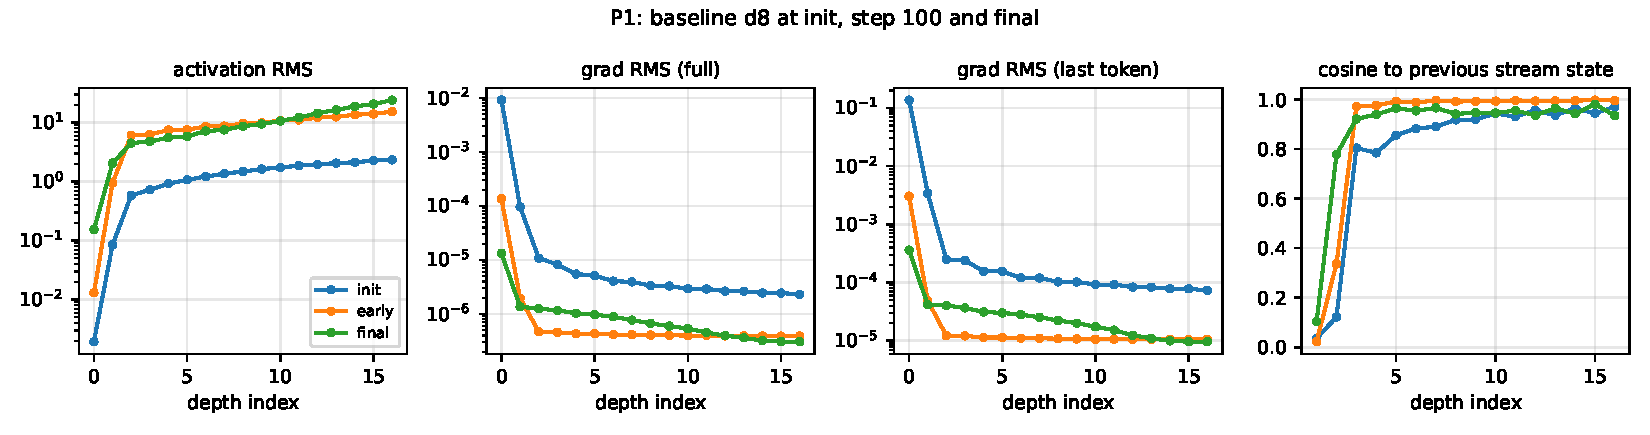
\includegraphics[width=\linewidth]{p1_d8_stages.pdf}
\caption{Baseline d8 at initialisation, step 100 and the final checkpoint.}
\label{fig:p1stages}
\end{figure}

\subsection{Attention patterns and sinks}
Figure~\ref{fig:p1attn} compares attention mass on the first token, mass on the query itself and mean lag with the uniform causal prefix baseline. Every trained model with residuals puts far more mass on the first token than uniform attention would: at position 1000 the baseline averages 0.08 on the first token (100 times uniform) and the no-prenorm and no-final-norm models 0.3 to 0.4. This is the attention sink. The mass on self flattens at 0.03 to 0.1 rather than decaying as $1/(t+1)$, and the mean lag is close to but below the uniform $t/2$, so the layers are a mixture of near uniform averaging heads, sink dominated heads and local heads. The no-residual model matches the uniform baseline exactly in all three statistics: its attention never learned anything. The two gated variants and the plain baseline have the smallest sinks (gated attention falls to 0.01 at the end of the context), consistent with the gate doing the job of switching heads off that the sink otherwise does. Without RoPE the sink is as strong as the baseline's but the model is 0.14 nats worse and its context test below shows that it depends on the first token to work at all.

\begin{figure}[h]\centering
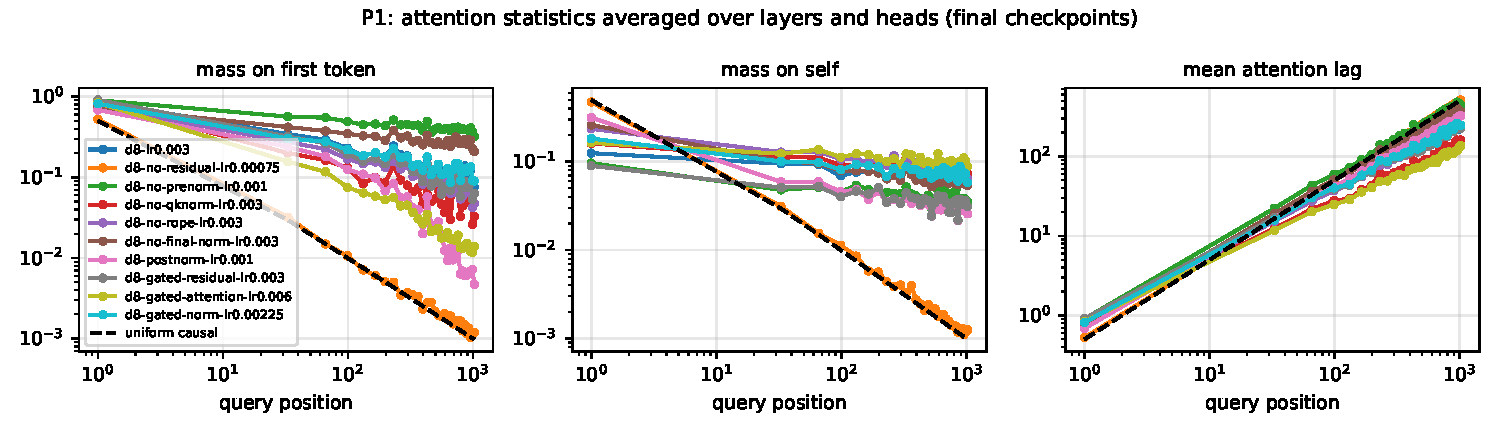
\includegraphics[width=\linewidth]{p1_attention.pdf}
\caption{P1 attention statistics on 32 query positions, averaged over heads and layers of the final checkpoints. Dashed: uniform causal prefix.}
\label{fig:p1attn}
\end{figure}

\subsection{Context use}
Figure~\ref{fig:p1ctx} reruns the last token prediction with only the $k$ most recent input tokens. The baseline loses 6.5 nats with one token of context, 1.7 with 16, 0.4 with 64 and under 0.1 with 256 or more, so the model relies on about 100 tokens for most of its loss but still gains measurably from the full window. Restoring the first token (a sink for every head) halves the penalty at short contexts. The no-RoPE model is the pathological case: without the first token its loss increase is 4.5 nats even with 512 recent tokens, and with the first token restored it is the model that recovers fastest. Its heads have no positional signal, so they use the first token as a fixed anchor and fail without it.

\begin{figure}[h]\centering
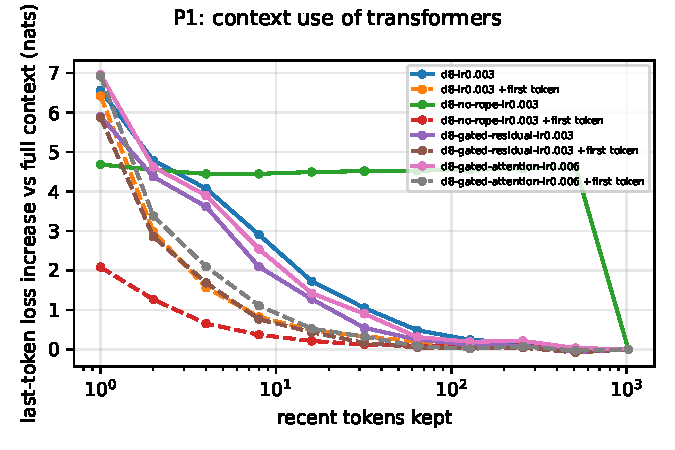
\includegraphics[width=.5\linewidth]{p1_context.pdf}
\caption{P1 context tests: increase of the last token loss over the full window loss, 64 validation sequences. Dashed lines restore the first token.}
\label{fig:p1ctx}
\end{figure}
